\documentclass[electronics,article,submit,pdftex,moreauthors]{Definitions/mdpi}

%=================================================================
% MDPI internal commands - do not modify
\firstpage{1}
\makeatletter
\setcounter{page}{\@firstpage}
\makeatother
\pubvolume{1}
\issuenum{1}
\articlenumber{0}
\pubyear{2026}
\copyrightyear{2026}
\datereceived{ }
\daterevised{ }
\dateaccepted{ }
\datepublished{ }

%=================================================================
% TikZ for architecture diagram; pgfplots for performance charts
\usepackage{tikz}
\usetikzlibrary{shapes.geometric,arrows.meta,positioning,fit,backgrounds,calc}
\usepackage{pgfplots}
\pgfplotsset{compat=1.18}
\setlength{\emergencystretch}{3em}
\newcommand{\orcidauthorA}{0009-0002-7781-7118}
\newcommand{\orcidauthorB}{0000-0001-8737-2402}
\newcommand{\orcidauthorC}{0000-0002-6832-4381}
\newcommand{\orcidauthorD}{0000-0002-7382-4276}
\renewcommand{\orcidA}{\href{https://orcid.org/0009-0002-7781-7118}{\orcidicon}}
\renewcommand{\orcidB}{\href{https://orcid.org/0000-0001-8737-2402}{\orcidicon}}
\renewcommand{\orcidC}{\href{https://orcid.org/0000-0002-6832-4381}{\orcidicon}}
\renewcommand{\orcidD}{\href{https://orcid.org/0000-0002-7382-4276}{\orcidicon}}
\Title{A Resilient and Low-Latency Cloud-Native Architecture for Real-Time Remote Video Production Using Open-Source Software}

\Author{Mart\'in Herranz-S\'anchez $^{1}$\orcidA{}, \'Alvaro Llorente-G\'omez $^{1,}$*\orcidB{}, Alberto del R\'io-Ponce $^{1}$\orcidC{} and David Jim\'enez-Bermejo $^{1}$\orcidD{}}

\AuthorNames{Mart\'in Herranz-S\'anchez, \'Alvaro Llorente-G\'omez, Alberto del R\'io-Ponce and David Jim\'enez-Bermejo}

\address{%
$^{1}$ \quad Departamento de Se\~nales, Sistemas y Radiocomunicaciones, Escuela T\'ecnica Superior de Ingenieros de Telecomunicaci\'on, Universidad Polit\'ecnica de Madrid, 28040 Madrid, Spain;
martin.herranz@alumnos.upm.es (M.H.S.); alvaro.llorente@upm.es (\'A.L.);
david.jimenez@upm.es (D.J.B.); alberto.delrio@upm.es (A.R.P.)}

\corres{Correspondence: alvaro.llorente@upm.es}

\abstract{%
Professional live video production remains constrained by dedicated hardware
switchers and proprietary desktop applications, which limit reproducibility,
headless operation, and deployment in research or small-broadcaster contexts.
This paper presents Voctomix~2.0, an extended and fully containerised version of
the open-source Voctomix live video mixer, built on GStreamer and validated
across four deployment scenarios from a single workstation to Kubernetes.
The system adds a real-time overlay and dual-text lower-third workflow with
automatic deactivation on cuts, a three-state stream blanker
(LIVE\,/\,PAUSE\,/\,NOSTREAM), Audio Follows Video automation, RabbitMQ AMQP
telemetry, and an eleven-service Docker Compose stack deployable with a single
command.
Performance was measured on Docker Compose and Minikube using four synthetic
1080p25 sources.
The Docker deployment sustained the workload at 38.8\% CPU and 10.1\% RAM, with
source-switching latency below 5~ms in all 30 measurements (median 1.5~ms).
A 31-minute stability run showed no CPU or memory growth, and a failed camera
container recovered in approximately 520~ms.
The system was also exercised in a CyberNEMO research-project deployment at
Universidad Polit\'ecnica de Madrid, validating the overlay, blanker, and
telemetry functions in a production-oriented setting.
}

\keyword{GStreamer; live video production; remote production; open-source; Docker; Kubernetes; video mixing; broadcast automation; real-time}

%%%%%%%%%%%%%%%%%%%%%%%%%%%%%%%%%%%%%%%%%%
    \begin{document}

%%%%%%%%%%%%%%%%%%%%%%%%%%%%%%%%%%%%%%%%%%
\section{Introduction}
\label{sec:introduction}

% \subsection{\hl{Background and motivation}}

The broadcast industry's transition from dedicated Serial Digital Interface (SDI)~\cite{smpte_sdi} infrastructure to IP based workflows has dramatically lowered the cost of signal transport, yet the mixing and compositing layer has remained anchored to proprietary hardware, where production suites combine switchers, control surfaces, routing, capture, monitoring, and site engineering, so costs scale rapidly from low-cost devices to capital-intensive installations~\cite{blackmagic_atem}.

They also tie organisations to vendor-specific hardware refresh cycles.

Software-Defined Video addresses this dependency by relocating the mixing and compositing function from fixed-purpose hardware into software processes running on commodity servers, connected over standard IP networks rather than dedicated SDI matrices; the same production logic that was previously bound to a specific chassis becomes deployable, replicable, and remotely operable on a laptop, a rack-mounted server, or a container orchestrated across a cloud cluster.

The Remote Integration Model (REMI) partially addresses the logistical dimension by concentrating mixing in a centralised IP-connected facility while cameras and contribution encoders remain on site, enabling production teams to work from any location with network connectivity~\cite{tmbroadcast_remi}; industry analysis confirms this transition toward cloud-native and containerised broadcast workflows is accelerating across the sector, driven by the same reproducibility and deployment-flexibility demands that motivate this work~\cite{haivision_broadcast_report_2025}. Even where REMI is adopted, on-site staff are still required to operate cameras and contribution encoders, and existing implementations are typically built on the same monolithic, vendor-specific software stacks as the hardware they replace, limiting the reproducibility and remote-operability gains REMI is meant to deliver.

Although software-based tools have significantly lowered the entry barriers to media production, current solutions exhibit critical architectural limitations for professional, cloud-orchestrated environments. On one hand, widely adopted open-source platforms like OBS Studio feature a monolithic design that couples capture, compositing, and output within a desktop application tailored for a single local operator rather than a headless, shared cloud deployment. On the other hand, professional suites like vMix impose prohibitive commercial licensing costs, strict operating system dependencies, and a complete lack of containerization support, excluding them from modern cloud infrastructures. While open-source frameworks like Voctomix pioneered a client–server architecture to decouple the media engine from the control interface, its earlier iterations lacked the robust features required for professional broadcast and cloud orchestration workflows, notably missing real-time telemetry channels, reproducible deployment paths, and advanced dynamic compositing capabilities.

% \subsection{Contributions of this work}

This paper presents a highly resilient, cloud-native remote video production architecture built on top of the open-source Voctomix 2.0 framework. Taking Voctomix 2.0 as our architectural baseline, we introduce key structural, operational, and telemetry-driven extensions designed to bridge the gap between lightweight open-source software and complex, proprietary broadcast systems. Furthermore, we conduct a comparative analysis evaluating our enhanced system against current industry-standard tools (specifically OBS Studio and vMix) under identical operational conditions. The principal contributions of this work are:

\begin{itemize}
\item An Enhanced, Production-Grade Extension Layer: We design and implement key features on top of the Voctomix 2.0 baseline, including automated Audio Follows Video (AFV) switching, dynamic multi-layer alpha overlays, and a stream blanking module operating at the compositor and audio-mixer level. These extensions are integrated modularly, proving that highly specific broadcast requirements can be customized without altering or destabilizing the low-level multimedia mixing engine.
\item A Decoupled Telemetry and Monitoring Framework: We introduce an asynchronous state exporter that translates GStreamer/TCP pipeline events into structured JSON lines, publishing them to a RabbitMQ message broker. This contribution enables non-intrusive, real-time auditing and automated multi-operator synchronization—a critical capability missing in standard open-source tools.
\item A Standardized, Reproducible Deployment Topology: We eliminate the manual configuration overhead typical of open-source multimedia software. By leveraging container network sharing, we supply a "plug-and-play" service stack and declarative Kubernetes manifests, proving that complex, low-latency broadcast environments can be orchestrated dynamically on standard cloud infrastructure.
\item A Rigorous Comparative Evaluation with Industry Standards: We subject our proposed architecture to empirical testing alongside OBS Studio and vMix. We present comparative metrics analyzing system resource footprints (CPU/RAM scaling from 1 to 4 camera sources), switching latencies, and failover resilience.
\end{itemize}

Taken together, this work demonstrates that an extended, cloud-native open-source architecture can match the operational capabilities of propietary environments, offering three key advantages to adopting organizations:

\begin{itemize}
    \item No licensing or platform lock-in: Our solution is completely platform-agnostic, running natively or standard Linux-based server infraestructure.
    \item True cloud orchestration vs desktop monolithics: While popular tools remain desktop-bound and designed for a single local operator, our extended architecture is fully container-native, allowing remote operators to control a headless, synchronized mixing pipeline provisioned on existing clusters in minutes.
    \item Highly customizable: Because the baseline is fully open-source, developers can inject custom plugins or adapt the TCP-based command protocol to implement specialized automation workflows, a level of control that proprietary black-box software entirely restricts.
\end{itemize}

The remainder of this paper is organised as follows: Section~\ref{sec:background} reviews related work in live video production systems and containerised media workflows. Section~\ref{sec:architecture} describes the Voctomix~2.0 system architecture, the deployment scenarios in which it was exercised, and the experimental setup and test plan used to evaluate it. Section~\ref{sec:results} reports validation results and performance metrics. Section~\ref{sec:discussion} discusses the findings, security considerations, limitations, and directions for future work. Section~\ref{sec:conclusions} presents the main conclusions.

%%%%%%%%%%%%%%%%%%%%%%%%%%%%%%%%%%%%%%%%%%
\section{Related Works}
\label{sec:background}

\subsection{Remote Video Production Standards and Protocol}

Remote production relies on a layered set of transport protocols suited to different stages of the signal path: for contribution, where quality and minimal latency are prioritised over reach, Secure Reliable Transport (SRT)
provides packet-loss recovery over UDP with sub-second latency, the de facto standard for camera-to-facility links~\cite{sharabayko2024_srt}; WebRTC, standardised by the W3C for real-time browser-based communication, achieves 100--500~ms latencies over UDP with built-in encryption (DTLS/SRTP), but its peer-to-peer signalling scales poorly to mass audiences, better suited to monitoring and return-feed channels than distribution~\cite{w3c_webrtc}; and RTMP, Adobe's legacy TCP-based ingest protocol, remains the most widely supported ingest format for platforms such as YouTube Live and Twitch despite its age, with 58\% adoption among broadcasters in 2025~\cite{haivision_broadcast_report_2025}. In cloud-hosted deployments, these protocols increasingly terminate at containerised ingest points rather than dedicated hardware encoders, so the transport and compute layers share the same commodity infrastructure, reducing the physical footprint of the contribution chain.

The contribution path feeding a software mixer is equally critical. Internet-facing contribution relies on SRT, WebRTC, and RTMP, intra-facility and local studio environments have shifted toward uncompressed IP standards, most notably SMPTE ST 2110. That is, professional broadcast has migrated from hardware SDI matrix routing under SMPTE ST~2022-6~\cite{smpte_st2022_6} towards uncompressed IP media via SMPTE ST~2110~\cite{smpte_st2110_20}, part of the broader industry shift toward sub-second glass-to-glass latency in live media streaming~\cite{bentaleb2023_live_latency}. Although ST 2110 offers ultra-low latency by splitting video, audio, and ancillary data into independent streams, it demands complex multicast network routing and strict  Precision Time Protocol (PTP)~\cite{ieee1588_2019} hardware synchronization.


% \subsection{The Evolution of Live Video Production: From Traditional to Remote and Virtualized Systems}
\subsection{Hardware-Defined vs. Software-Defined Video Mixing}
\label{sec:background:production}

This section traces the transition from hardware-defined production, where mixing and compositing are bound to a dedicated physical switcher, to the software-defined model introduced in Section~\ref{sec:introduction}, in which the same function runs as a portable process on general-purpose infrastructure.

Production switchers have traditionally been dedicated hardware units: the Blackmagic ATEM family ranges from a few hundred dollars for compact switchers to roughly \$15{,}000 for high-end units such as the ATEM~4~M/E Constellation 4K~Plus, with comparable Ross Video systems in a similar tier~\cite{blackmagic_atem}, and once combined with SDI matrix routing, specialised control surfaces, redundant infrastructure, and on-site engineering teams, complete production facilities reach hundreds of thousands to millions of dollars, excluding small-scale broadcasters, academic institutions, and research groups from professional live production.

Software mixers lower the financial barrier but introduce other limitations: OBS Studio provides free capture, compositing, and streaming with WebSocket-based automation~\cite{obs_studio,obs_websocket}, but couples production functions in a desktop application for direct operator interaction rather than a headless server-side mixer shared by multiple remote clients; vMix supports multi-source mixing and 4K output, but its commercial licence (from \$60 to over \$1\,000 per seat), mandatory Windows platform, and absence of a container runtime path exclude it from Linux infrastructure and reproducible cloud deployments~\cite{vmix_software}. 

REMI partially addresses the logistical barrier by centralising mixing in an IP-connected facility, but existing implementations rely on the same proprietary hardware-software stacks~\cite{tmbroadcast_remi}; large-scale deployments confirm the approach's viability, as with Olympic Broadcasting Services' REMI workflows at the Tokyo~2020 Games~\cite{obs_tokyo_2021} and Telef\'onica Servicios Audiovisuales and Appear's SRT-based contribution network for LaLiga~\cite{tsa_laliga_srt_2025}, but none of these solutions expose a structured API, operate without a display server, or integrate natively with container orchestration.

GStreamer is a plugin-based multimedia framework that models media processing as directed graphs of elements connected by
pads~\cite{gstreamer_docs}, with a bus-based architecture, caps negotiation, and hardware-accelerated elements (VA-API, NVENC) well suited to modular, real-time processing graphs inspectable at runtime. FFmpeg provides extensive codec and format conversion support but targets file-based or single-stream command-line workflows rather than multi-source live compositing.

The third and current phase of this evolution virtualises the mixing function itself: instead of a fixed facility, the production pipeline becomes a set of container images that can be instantiated on any sufficiently provisioned host, from a laptop to a managed cloud cluster~\cite{kubernetes_burns2016}. This has a direct architectural consequence for mobility: a production pipeline packaged this way is not tied to a specific physical installation the way an SDI matrix or a hardware switcher is, and the same container images and manifests that run in a lightweight local cluster during development~\cite{minikube_docs} are, in principle, redeployable unmodified on any conformant Kubernetes cluster, including a remote or cloud-hosted one. 


\subsection{Cloud-Native and Orchestrated Media Processing}

Real-time multimedia processing has traditionally run as long-lived, tightly coupled processes on dedicated on-premises servers, with codecs, drivers, and library versions matched by hand to a specific host rather than packaged for portable, repeatable execution.

Containerisation directly targets this fragility: Boettiger showed that packaging a full dependency graph, including library versions, codecs, and runtime configuration, into a Docker image restores computational reproducibility across otherwise incompatible hosts~\cite{boettiger2015_docker_reproducibility}; Docker Compose extends this to multi-service topologies by declaratively specifying inter-service networking and startup ordering, directly applicable to the producer-consumer model of a mixer with multiple camera ingestion services.

Orchestrating this kind of workload introduces requirements that general-purpose container platforms were not originally designed for, including bounded scheduling latency, access to GPU or capture-card hardware via device plugins, and headless operation without a display server; because privileged hardware access widens the container attack surface, these deployments also inherit the broader security trade-offs surveyed by Jarkas et al. for container-based infrastructure~\cite{jarkas2025_container_security}. The closest comparable evaluation is that of Shih et al., who benchmarked a DeepStream-based stream service on containerised edge infrastructure against a native deployment, quantifying the containerisation overhead for real-time media processing~\cite{shih2025_containerized_gstreamer}.



\subsection{Open-Source Video Mixers: The Voctomix Framework}
\label{sec:background:voctomix}

Voctomix, originally developed by the C3VOC team for the Chaos Communication Congress, was the first open-source system to apply a true client--server split to live video production: a GStreamer-based mixing engine (\texttt{voctocore}) decoupled from an operator GUI (\texttt{voctogui}) over a TCP control channel~\cite{voctomix_github,c3voc_voctomix_origin}, enabling multiple remote operators to share a single mixer instance on a dedicated headless server. On a previous work~\cite{delRio2025}, it was demonstrated on real-world deployment its operational viability by deploying Voctomix~v1.3 as the Production Core of a quality-aware live streaming pipeline during a large-scale sporting event with geographically separated teams, validating the client--server model under real broadcast conditions and providing the baseline from which Voctomix~2.0 is derived.

The closest comparable open-source project is Nageru, a GPU-accelerated live mixer developed for FOSDEM and driven by a Lua-scripted theme, restricted to DeckLink and UltraStudio capture hardware~\cite{nageru_project,gunderson2016_nageru_fosdem}; because Nageru has no client--server split, mixing and operator control run as a single process on one machine, in contrast to Voctomix's decoupled engine and GUI, which allow the mixer to run headless on a remote server while multiple operators connect independently over the network. This difference illustrates a broader pattern in the open-source live-mixing space: projects have so far specialised either in tight, single-host integration with specific capture hardware, as with Nageru, or in network-controllable, headless operation, as with Voctomix, rather than combining both.


\subsection{Qualitative Comparison and Research Gap}
% \label{sec:results:comparison}

To clearly delineate the structural limitations of current live production systems, Table~\ref{tab:comparison} positions our proposed extended framework against the prominent industry alternatives reviewed in this section: OBS~Studio~\cite{obs_studio}, vMix~\cite{vmix_software}, and the Blackmagic ATEM family~\cite{blackmagic_atem}.

\begin{table}[H]
\caption{Feature comparison of live video production tools.\label{tab:comparison}}
\small
\begin{tabularx}{\textwidth}{XCCCC}
\toprule
\textbf{Feature} & \textbf{Voctomix 2.0} & \textbf{OBS Studio} & \textbf{vMix} & \textbf{ATEM}\\
\midrule
Licence cost           & Free       & Free       & \$60--1\,000  & \$295--15\,k (HW)\\
Open-source            & Yes        & Yes        & No            & No\\
Linux headless server  & Yes        & No         & No            & N/A\\
Containerisable        & Yes        & Partial    & No            & N/A\\
Machine-readable API   & TCP (text) & WebSocket  & TCP (limited) & SDK (proprietary)\\
Client--server split   & Yes        & No         & No            & No\\
Multi-operator         & Yes        & No         & No            & No\\
AMQP telemetry         & Yes        & No         & No            & No\\
K8s deployable         & Yes        & No         & No            & N/A\\
\bottomrule
\end{tabularx}
\end{table}

As highlighted by this matrix, the proposed extended architecture is the only system that combines zero licensing costs, headless Linux operation, native containerization, and a structured machine-readable API within a true client--server topology capable of sustaining multi-operator workflows. Each established alternative lacks at least one of these technical pillars, resulting either in a desktop-bound single-operator bottleneck (OBS Studio), prohibitive licensing fees tied to a mandatory Windows runtime (vMix), or closed hardware ecosystems that prevent software-driven automation and remote cloud orchestration (the ATEM family). This architectural void defines the precise research gap that motivates the proposed system design.

%%%%%%%%%%%%%%%%%%%%%%%%%%%%%%%%%%%%%%%%%%
\section{Methodology}
\label{sec:architecture}

\subsection{System Architecture}
\label{sec:architecture:overview}

Voctomix~\cite{voctomix_github,c3voc_voctomix_origin}, originally developed by the C3VOC team for the Chaos Communication Congress, was the first open-source system to apply a true client--server split to live video production: a GStreamer-based mixing engine (\texttt{voctocore}) decoupled from an operator GUI (\texttt{voctogui}) over a TCP control channel, enabling multiple remote operators to share a single mixer instance on a dedicated headless server. On a previous work~\cite{delRio2025}, it was demonstrated on real-world deployment its operational viability by deploying Voctomix~v1.3 as the Production Core of a quality-aware live streaming pipeline during a large-scale sporting event with geographically separated teams, validating the client--server model under real broadcast conditions and providing the baseline from which Voctomix~2.0 is
derived.

Voctomix~2.0 follows a strict client--server separation (Figure~\ref{fig:architecture}). The processing server, \texttt{voctocore}, hosts a GStreamer multimedia pipeline that accepts up to six (by default) simultaneous video/audio input streams over TCP, performs compositing and mixing, and delivers the programme signal on port~15000. The operator interface, \texttt{voctogui}, is a GIMP Toolkit (GTK)~3 desktop application that connects to \texttt{voctocore} over a dedicated control channel on port~9999. When preview encoding is enabled, per-source JPEG preview streams are served on ports~14000--14005, while the mixer preview and programme output are exposed separately on ports~12000 and~15000, respectively. Multiple \texttt{voctogui} instances may connect simultaneously, enabling multi-operator workflows without restarting the mixing engine.


\begin{figure}[H]
\begin{center}
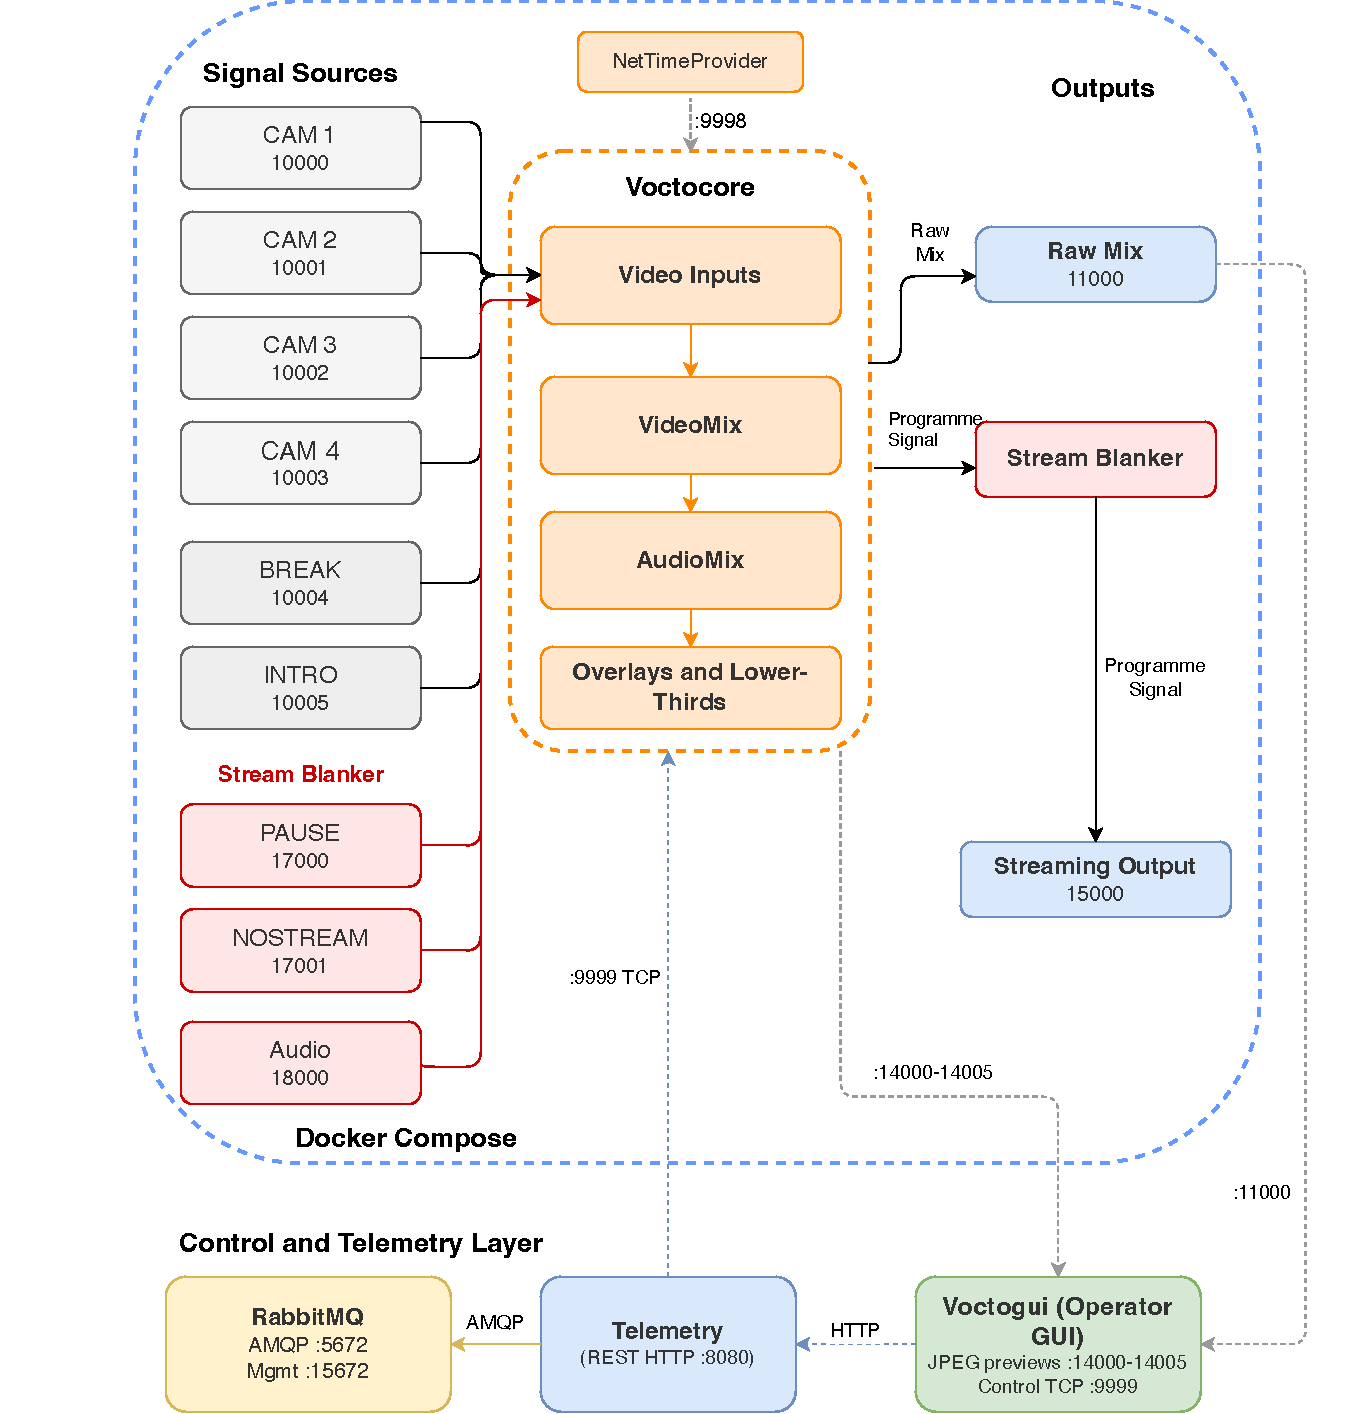
\includegraphics[width=\textwidth]{figures/system_architecture.pdf}
\end{center}
\caption{Voctomix~2.0 system architecture.\label{fig:architecture}}
\end{figure}

% \subsubsection{voctocore: the Processing Core}
% \label{sec:architecture:voctocore}

% \textbf{GStreamer pipeline design.}
\texttt{voctocore} constructs a single GStreamer pipeline at startup, static after initialisation.
The internal video format is 8-bit YUV (I420, 4:2:0) at 1920$\times$1080 pixels and 25~fps, chosen as the native raw format most GStreamer elements and distribution-oriented H.264 encoders consume without an intermediate colour-space conversion, and because its lower memory and bandwidth footprint compared with broadcast-grade 4:2:2 or 10-bit formats matches this work's goal of running on commodity, containerised infrastructure rather than dedicated capture hardware; audio is 16-bit linear PCM (S16LE) at 48~kHz, stereo, negotiated at source boundaries via GStreamer caps and maintained without intermediate re-encoding. Inter-module data flow uses GStreamer \texttt{appsrc}/\texttt{appsink} pairs, allowing each processing module (video mixing, audio mixing, overlay, and stream blanking) to run as an independent Python object without pipeline relinking at runtime. A \texttt{NetTimeProvider} element broadcasts a GStreamer network clock over UDP port~9998, to which all camera-ingest containers synchronise for presentation-time alignment.

% \textbf{Source management.}
% \label{sec:architecture:voctocore:sources}

Six logical source slots are defined: \texttt{cam1}--\texttt{cam4} for live camera feeds, \texttt{break} for a pre-recorded loop, and \texttt{intro} for an opening sequence, each listening on a dedicated TCP port (10000--10005) with its source plugin selected via a configuration parameter. The default network plugin accepts a Matroska-wrapped raw stream from an upstream FFmpeg process, which decodes and re-muxes each
camera feed in the Docker deployment; a static-image plugin loops a PNG or JPEG for break and intro in native deployments, and a DeckLink plugin covers hardware SDI capture.

% \textbf{Composite modes and video mixing.}
% \label{sec:architecture:voctocore:composites}

The video mixing module maintains two logical channels, A and~B, updating the GStreamer \texttt{compositor} element's pad offsets, dimensions, and alpha values on each source-switch command, with mode changes taking effect at the next buffer boundary for a clean hard cut.

Four primary composite modes are exposed in the GUI (Figure~\ref{fig:composites}): \textit{Fullscreen} (single source, full resolution), \textit{Picture-in-Picture} (source~B in a configurable corner, approximately 26\% of frame width), \textit{Side-by-Side} (equal half-width), and \textit{Lecture} (75\% of the
frame for source~A, 23\% for source~B). Internal variants, a 4:3-constrained Lecture layout and a horizontal mirror modifier for PIP and Lecture, extend these four without exposing separate primary modes.

\begin{figure}[H]
\begin{center}
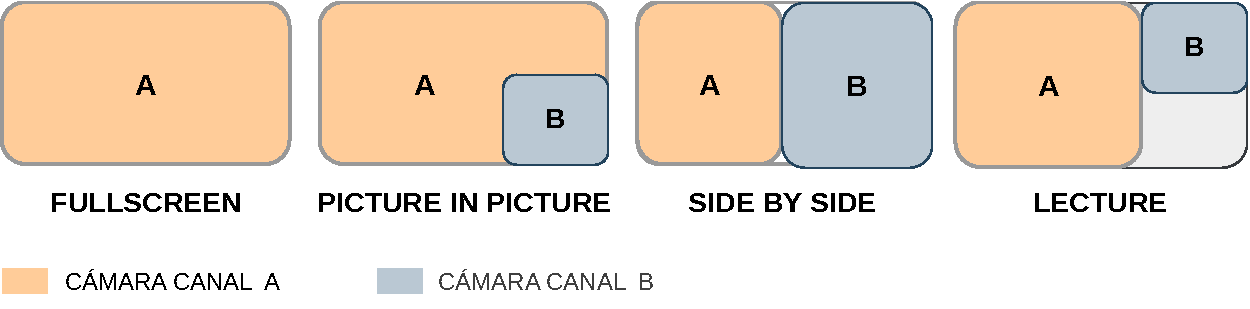
\includegraphics[width=0.81\textwidth, trim=0 30 0 0, clip]{figures/composites_diagrama}
\end{center}
\caption{Geometric layout of the main composite modes supported by the
video mixing module.\label{fig:composites}}
\end{figure}

% \textbf{Audio Follows Video.}
% \label{sec:architecture:voctocore:afv}

The audio mixing module implements AFV. When the active source~A changes, it sets the corresponding GStreamer \texttt{volume} element to unity gain and all other channels to silence via a direct property
assignment, with no intermediate ramp. \texttt{voctogui} issues this switch in the same control-protocol message as the \texttt{cut} or \texttt{transition} command, so the active audio channel always matches the active video source without manual operator adjustment. AFV operates independently of the composite mode and re-engages automatically on every source switch, though operators can override volumes manually through the GUI between switches.

% \textbf{Output control: stream blanker.}
% \label{sec:architecture:voctocore:blanker}

The stream blanker controls what is delivered to the programme output (port~15000) independently of the internal mixing state, using GStreamer \texttt{compositor} elements to choose among three signal paths: \texttt{LIVE} passes the mixed signal through unmodified; \texttt{PAUSE} routes a static image loop (port~17000) with background audio (port~18000), allowing hold content to play while the internal mix continues off-air; and
\texttt{NOSTREAM} delivers a silent black frame, cutting the output entirely. State transitions occur at the GStreamer buffer boundary for clean hard cuts, with the blanker state reflected in real time on the GUI toolbar and included in every telemetry event.

% \textbf{Overlay system.}
% \label{sec:architecture:voctocore:overlay}

The overlay system composites graphical lower-thirds and text annotations over the programme mix in real time, using a GStreamer \texttt{gdkpixbufoverlay} element for PNG graphics and two independent \texttt{textoverlay} elements, typically a name and a role or affiliation, each separately configurable in font, size, colour, and position. Fade-in/fade-out linearly animate the \texttt{alpha} property over a configurable duration (300~ms by default), and the overlay is automatically deactivated on every source cut: \texttt{voctogui} issues
\texttt{show\_overlay false} before forwarding any \texttt{set\_video\_a} or \texttt{set\_composite\_mode} command, ensuring lower-thirds never persist across unintended cuts.

% \subsubsection{voctogui: the Control Interface}
% \label{sec:architecture:voctogui}

Finally, \texttt{voctogui} is a GTK~3 desktop application providing the operator interface for the mixing session, running an asyncio event loop alongside the GTK main loop with non-blocking TCP I/O to \texttt{voctocore} so the
interface remains responsive under network latency. The window is divided into three panels (Figure~\ref{fig:voctogui}): a source preview column with JPEG thumbnails refreshed at the \texttt{voctocore}
output framerate (ports~14000--14005 when enabled, separate from the mixer preview and programme streams on ports~12000 and~15000); a central toolbar with source~A/B selectors, a composite-mode drop-down, LIVE/PAUSE/NOSTREAM blanker buttons, and an overlay control panel; and the state exporter.

\begin{figure}[H]
\begin{center}
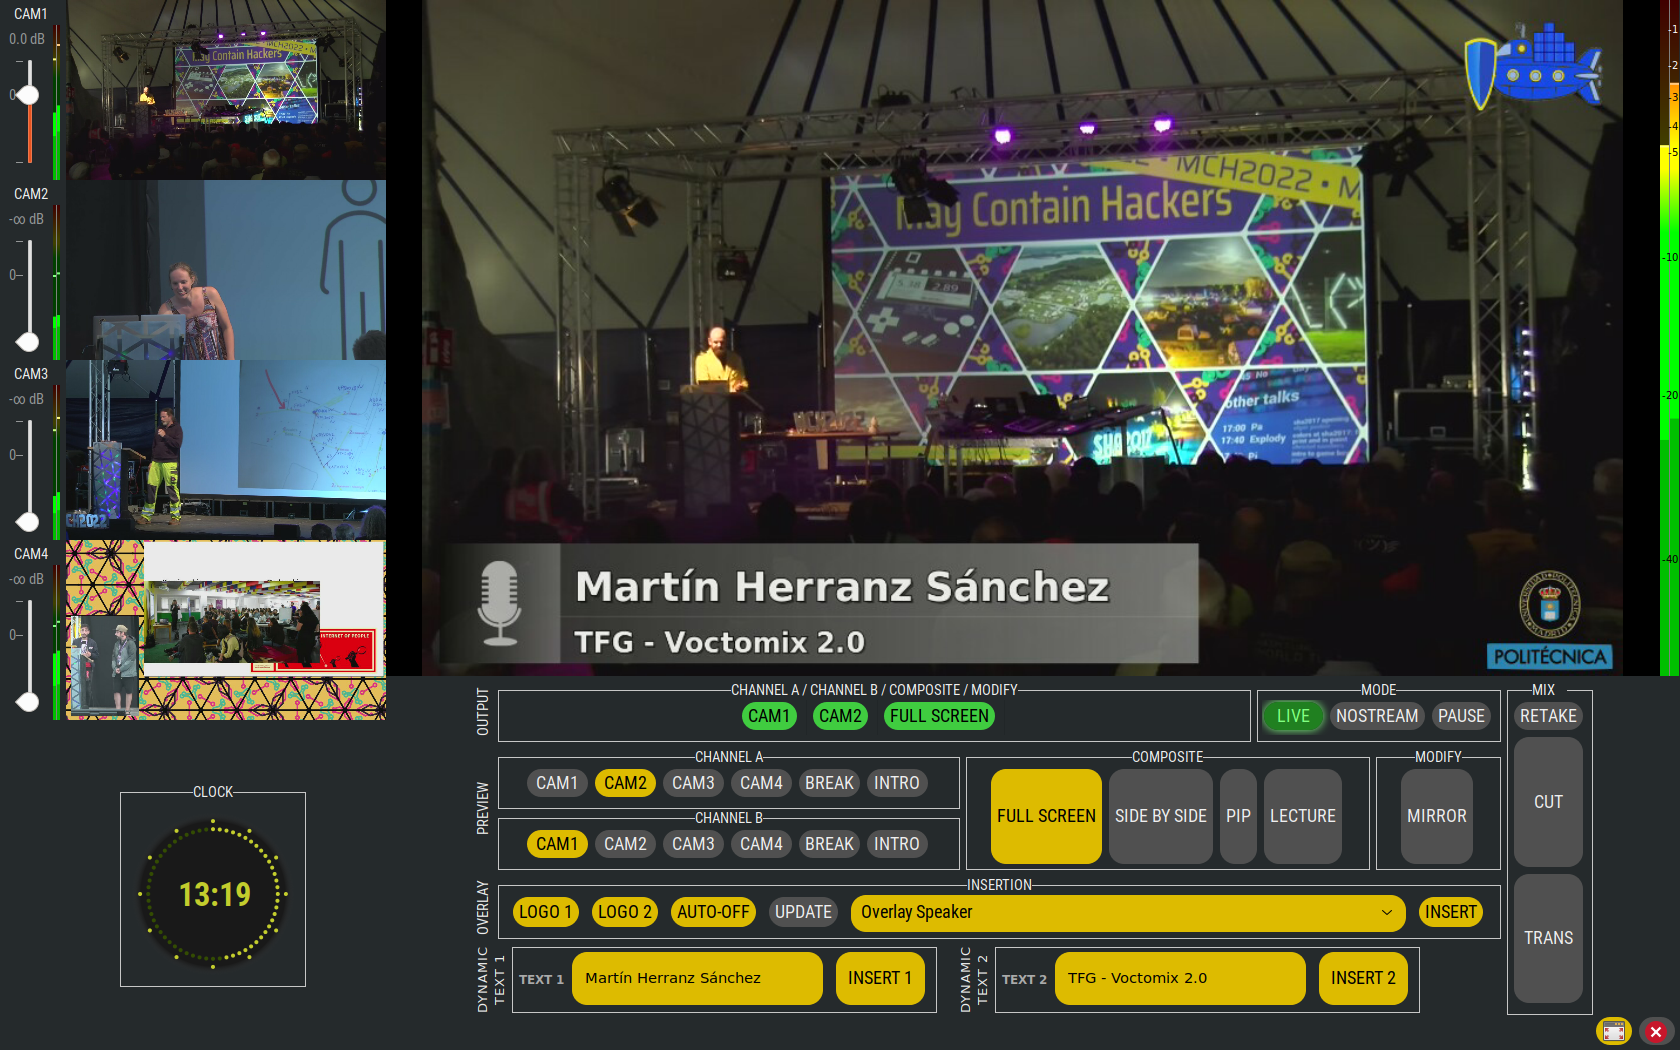
\includegraphics[width=0.90\textwidth]{figures/voctogui_screenshot}
\end{center}
\caption{The \texttt{voctogui} operator interface.\label{fig:voctogui}}
\end{figure}

% \subsubsection{TCP Control Protocol}
% \label{sec:architecture:protocol}

All mixer control is carried over a line-delimited ASCII protocol on TCP port~9999: each command is a single UTF-8 line, validated and executed by the server, which broadcasts a response event to \emph{all} connected
clients so multiple \texttt{voctogui} instances share a consistent view of the mixer state without a separate synchronisation mechanism. The core command set assigns source slots to channel~A or~B (\texttt{set\_video\_a}, \texttt{set\_video\_b}), changes the layout (\texttt{set\_composite\_mode}), toggles the overlay (\texttt{show\_overlay}), and changes the blanker state (\texttt{set\_stream\_blank}); commands with invalid arguments return an \texttt{error} event to the originating client only. The protocol is intentionally minimal: any scripted client, such as a cron job, a web backend, or an automation system, can control the mixer with a
single TCP socket and standard line I/O.

% \subsubsection{Telemetry and Monitoring}
% \label{sec:architecture:telemetry}

Observability was discussed as a recognised gap in distributed, where the difficulty of correlating state across independently scheduled services complicates outage detection and troubleshooting~\cite{usman2022_observability_microservices}. The telemetry subsystem addresses this for Voctomix~2.0 by exporting the complete mixer state to external systems without modifying the
\texttt{voctocore} core. The state exporter collects state from the live \texttt{voctogui} widget tree every second and publishes it through two paths depending on deployment mode: in native deployments, it appends JSON Lines records to a local session log for post-event analysis; in Docker deployments, it HTTP-POSTs
the same JSON object to the telemetry service (port~8080), which forwards the payload to a RabbitMQ AMQP exchange.

Two message types are published: \texttt{CHANGE} events are emitted immediately on any state transition (source switch, mode change, blanker or overlay toggle), enabling sub-second reaction latency in downstream consumers; \texttt{STATE} events are published periodically every five seconds as a heartbeat, allowing consumers to detect stale connections and reconstruct state after a reconnection. During the CyberNEMO integration, downstream project queues bound to the RabbitMQ exchange consumed Voctomix telemetry events in real time, confirming
the viability of the publish/subscribe model under an external consumer. The separation of change-driven and periodic events decouples monitoring freshness from polling rate, and the AMQP binding model allows any number
of external subscribers, such as dashboards, alerting systems, or recording services, to consume events without modifying the application.

% \subsection{Deployment Scenarios}
% \label{sec:deployment}
\subsection{Experimental Setup}

To evaluate the performance, scalability, and resilience of our extended cloud-native architecture against traditional production suites, we established a controlled benchmarking environment. The system was evaluated across three distinct deployment topologies of increasing virtualization complexity, using standardized high-definition video feeds under identical hardware constraints.

All experiments were conducted on a dedicated high-performance workstation to eliminate external network jitter and virtualization noise. Table~\ref{tab:testenv} details key hardware and software dependency and versions utilized for the evaluation.

\begin{table}[H]
\caption{Test environment and software versions.\label{tab:testenv}}
\begin{tabularx}{\textwidth}{lX}
\toprule
\textbf{Component} & \textbf{Specification}\\
\midrule
CPU              & Intel Core i9-10900 @ 3.70\,GHz (10 cores / 20 threads)\\
RAM              & 128\,GB DDR4\\
Operating system & Ubuntu 22.04.5 LTS\\
Docker           & Engine 29.1.3 / Compose 2.37.1\\
Kubernetes       & Minikube v1.38.1, single-node / kubectl v1.36.0\\
Runtime          & GStreamer 1.20 / Python 3.10\\
\bottomrule
\end{tabularx}
\end{table}

To analyze the performance overhead introduced by different virtualization and orchestration layers, the proposed extended pipeline was deployed in three distinct scenarios:

\begin{itemize}
    \item Local Native Deployment: All components—including voctocore, voctogui, and the four FFmpeg camera ingest subprocesses—run as bare-metal OS processes on a single host. This scenario establishes the absolute performance baseline, running natively without containerization or virtualized network layers.
    \item Docker Compose Stack: The pipeline is modularized into an 11-container microservice stack. To bypass Docker's virtual-Ethernet bridge overhead, camera containers utilize network\_mode: service:voctocore. This places them directly within the core mixer’s network namespace, routing all raw video traffic through the local loopback interface and exposing the necessary TCP ports on localhost.
    \item Kubernetes Orchestration: The central mixing architecture is declared as a multi-container Pod (\texttt{studio}) and scheduled on a single-node local Kubernetes cluster (Minikube). The core and its four camera ingest containers run as sidecars sharing the same network namespace. This design replicates the low-overhead loopback routing of the Docker Compose stack while exercising the same ConfigMap and Persistent Volume Claim primitives a multi-node production cluster would also rely on for configuration and telemetry state persistence.
\end{itemize}

\begin{figure}[H]
\centering
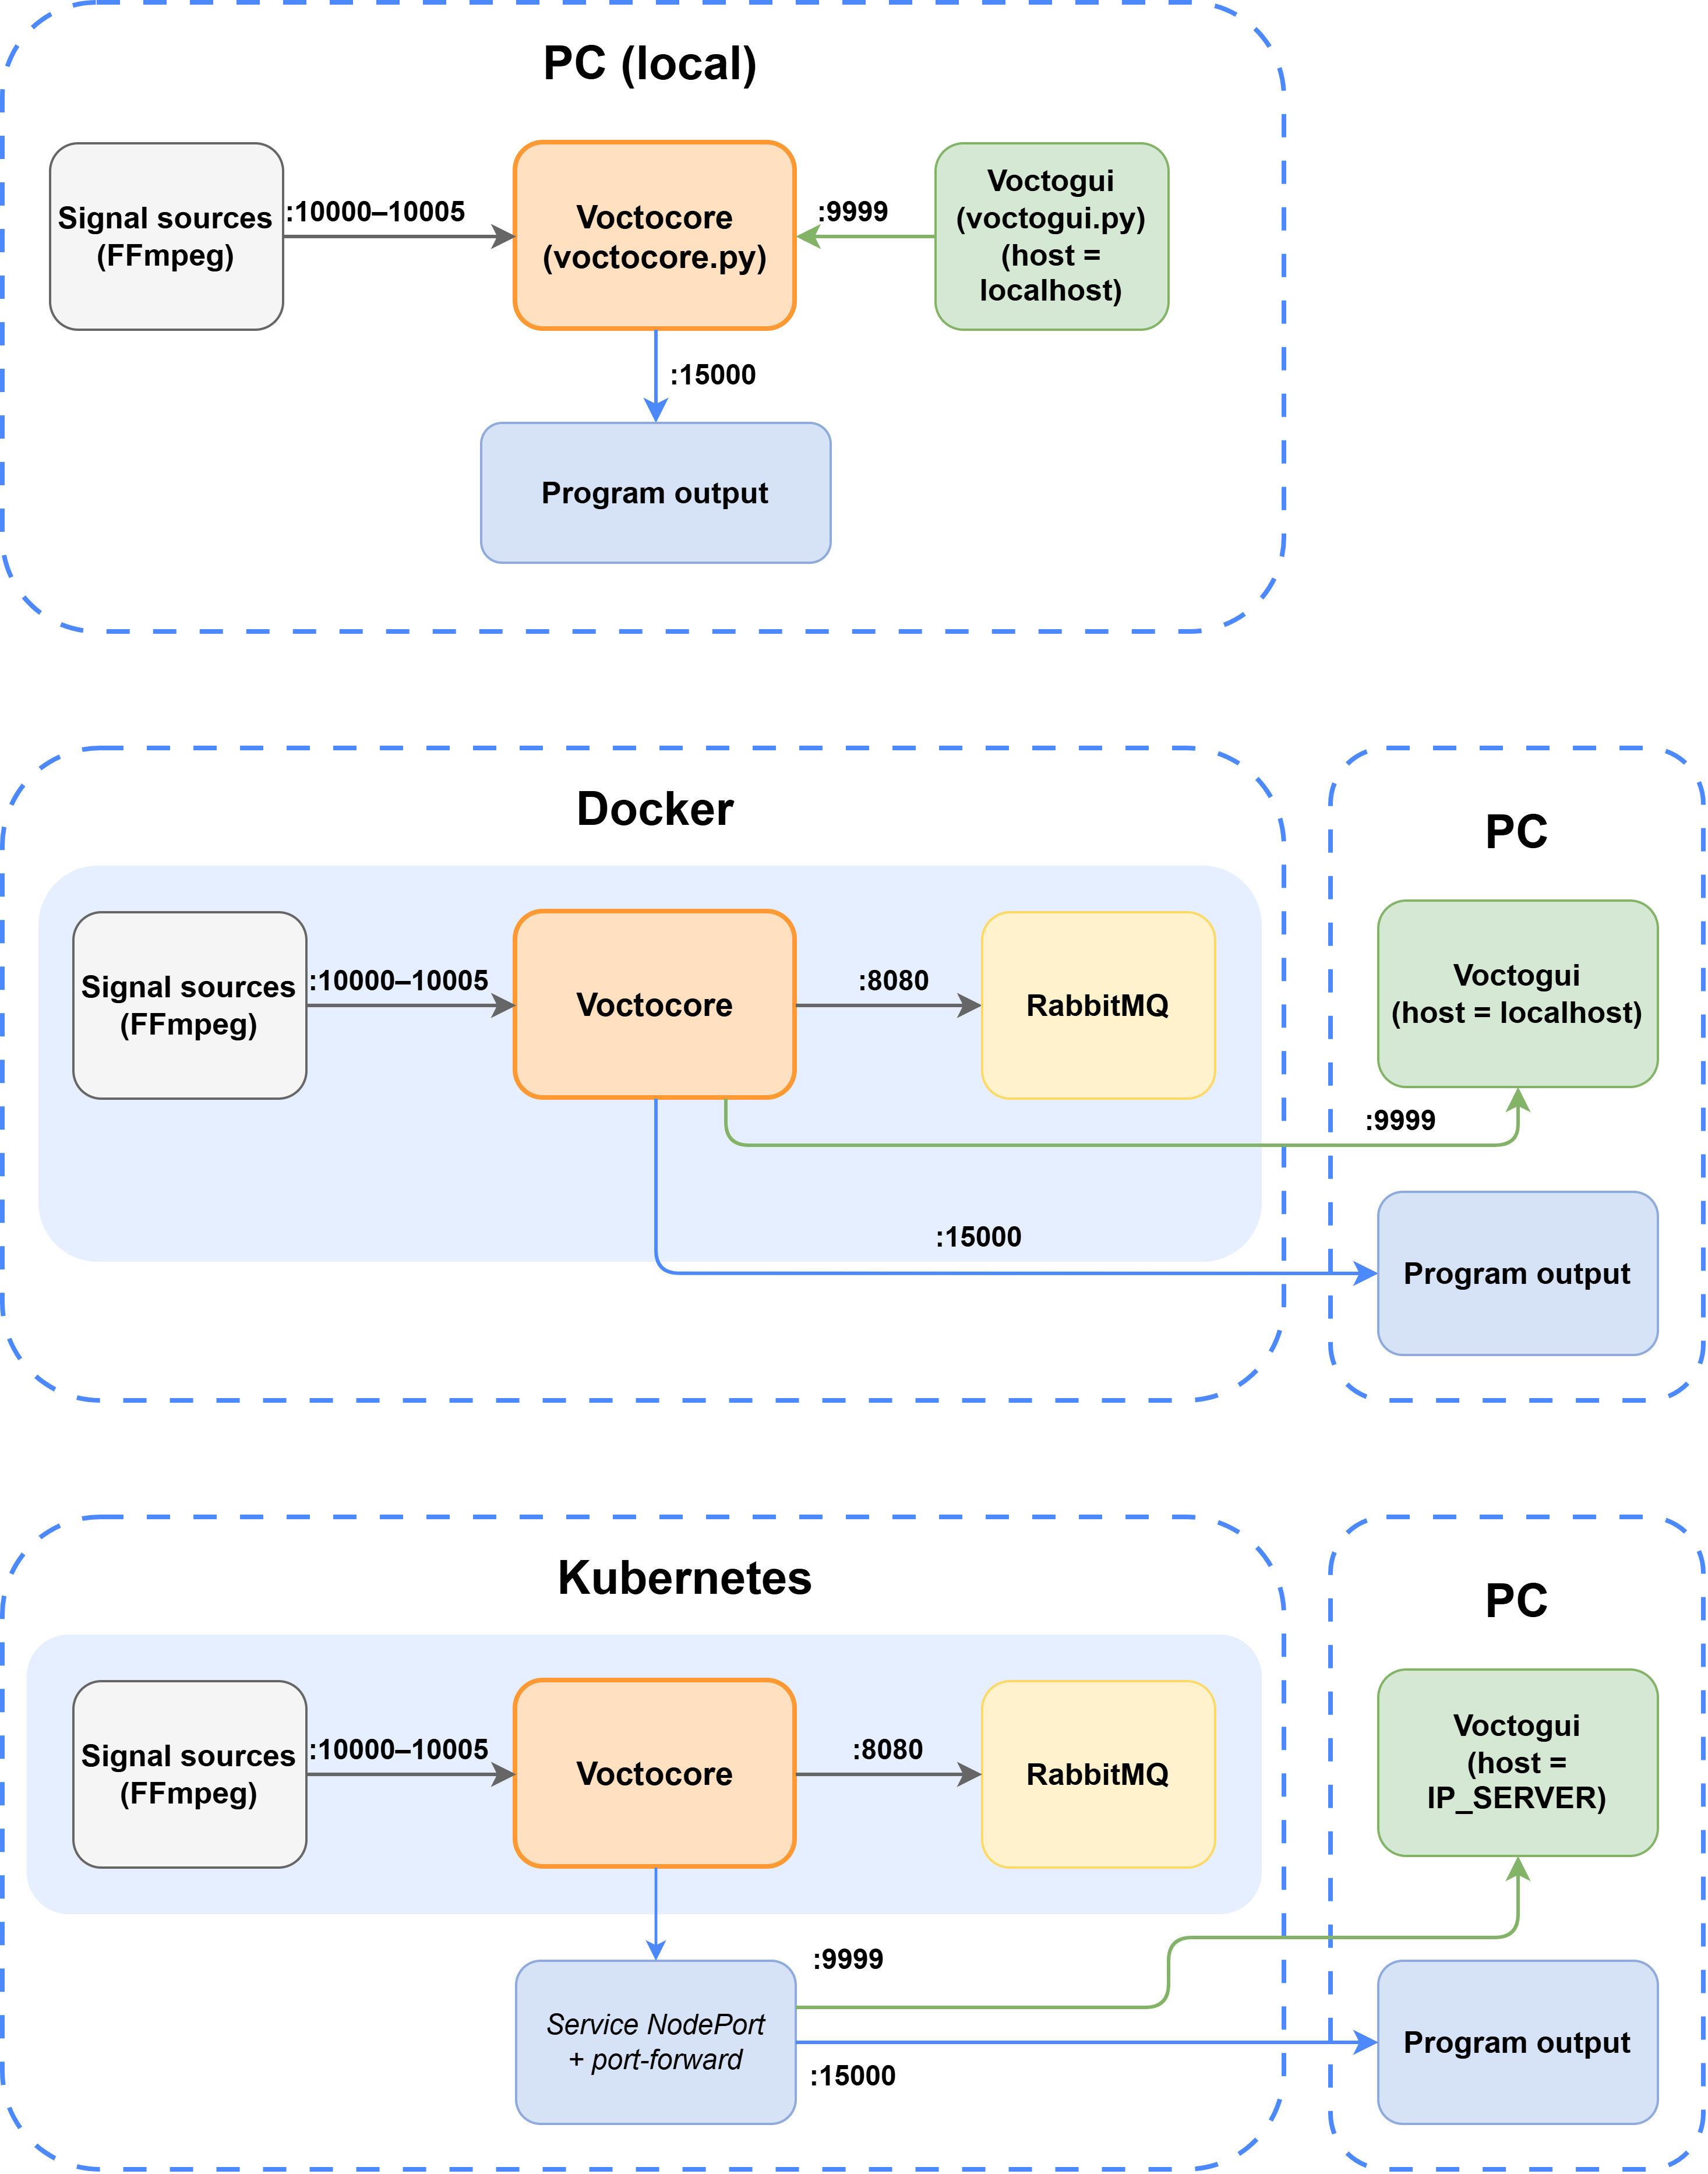
\includegraphics[width=0.85\textwidth]{figures/scenarios.png}
\caption{Architectural and networking layout of the three evaluated deployment topologies: (\textbf{top}) Local native setup on a single host process environment; (\textbf{middle}) Containerized microservice stack via Docker Compose with shared network namespace; and (\textbf{bottom}) Orchestrated multi-container Pod deployment within a Kubernetes cluster using port-forwarding for remote operator control.}
\label{fig:deployment_scenarios}
\end{figure}

From a deployment and networking perspective, the three evaluated topologies differ significantly in orchestration complexity, though they share an underlying low-overhead communication design (Figure~\ref{fig:deployment_scenarios}). In the local native setup (Figure~\ref{fig:deployment_scenarios}, top), all processes are executed on a single host PC, relying on automatic LAN IP detection to establish loopback TCP connections without container overhead. The Docker Compose scenario elevates this architecture to a container microservice stack, utilizing a single command to orchestrate startup dependencies and automatic service restarts. To eliminate virtual-bridge network overhead, the camera containers are mapped to \texttt{voctocore}’s network namespace, forcing all high-bandwidth traffic through \texttt{localhost}. Finally, the Kubernetes deployment schedules this same topology onto a single-node local cluster (Minikube), exercising the same Pod, ConfigMap, and PersistentVolumeClaim primitives a multi-node production cluster would also rely on: \texttt{voctocore} and the ingest engines run as sidecars within a single \texttt{studio} Pod, using localised port-forwarding for operator control and a dedicated PersistentVolumeClaim to isolate telemetry state.

This multi-scenario approach directly highlights the structural differences between our proposed architecture and competing platforms. While commercial software like vMix is locked to bare-metal Windows environments and OBS Studio operates strictly as a local desktop monolith, our system is evaluated across topologies ranging from a local developer machine to a Kubernetes-orchestrated deployment without modifying the core codebase.

Performance data was collected during active 5-minute broadcast runs under a constant load of four concurrent HD video sources ($1920\times1080$ at $25\text{ fps}$). To ensure statistical accuracy, the first 30 seconds of each run were treated as system warm-up and excluded from the analysis. 

The metrics were acquired and computed using the following telemetry and instrumentation mechanisms:

\begin{itemize}
    \item System Resource Utilization: CPU usage percentage and RAM footprints were sampled at $0.2\text{ Hz}$ (every 5 seconds) directly from the STATE events emitted asynchronously by our telemetry exporter.
    \item Energy Consumption: CPU-package power draw was calculated by reading energy deltas from the Intel Running Average Power Limit (RAPL) interfaces during active mixing operations.
    \item Switching and Transition Latency: The latency of scene changes (e.g., PiP, Side-by-Side) was calculated by computing the delta between the command timestamp sent by the controller and the corresponding acknowledgement returned over the same TCP control channel (\texttt{video\_status} for source switches, \texttt{composite} for layout transitions), reflecting command-processing latency at the control-protocol layer.
    \item Failover and Self-Healing Resilience: To benchmark system reliability against typical network/camera dropouts, a script forcibly terminated the container of the primary camera source (cam1). The time elapsed between the termination signal and the container being reported healthy again, based on the control-port liveness healthcheck, was measured as a proxy for the self-healing recovery time.
\end{itemize}

\subsubsection{Uncompressed Internal Transport Bandwidth}
\label{sec:results:bandwidth}

The video sources used in this evaluation arrive over the network already compressed, H.264-encoded recordings drawn from the CCC media archive in the Docker demonstration setup, or, in a native deployment, as uncompressed SDI captured locally via a DeckLink card. In either case, an FFmpeg process (or the native capture path) decodes or receives each source once and forwards it to \texttt{voctocore} as raw, uncompressed I420 frames, since compositing two or more video streams together requires operating on decoded pixel data rather than on independently encoded bitstreams. This decode-once, mix-raw, encode-once pattern is not specific to Voctomix: hardware switchers such as the Blackmagic ATEM family and software mixers such as OBS Studio and vMix all operate on uncompressed frames internally between input decoding and output encoding, so the bandwidth figure below characterises this class of system in general rather than a design choice unique to this work.

Each source stream in uncompressed I420~4:2:0 at 1920$\times$1080\,px and 25\,fps
carries:
\[
  B = \frac{1920 \times 1080 \times 1.5 \times 25}{10^6}
    \approx 77.8\ \text{MB/s} \approx 622\ \text{Mbps}.
\]

Bandwidth scales linearly with the number of active sources: with four
simultaneous sources the aggregate internal traffic is approximately
2.49~Gbps.
Because this volume exists only between the decoder and \texttt{voctocore}, it
circulates entirely over the loopback interface (native) or the Docker
internal bridge (\texttt{network\_mode:~service:voctocore}), and never
traverses a physical network interface or represents actual contribution
bandwidth; the external, network-facing bitrate remains whatever the
compressed source codec requires, a few Mbps per H.264 source, several
orders of magnitude below the internal figure.

This internal bandwidth requirement nonetheless imposes an architectural
constraint: the \texttt{network\_mode:~service:voctocore} pattern (or
equivalent pod co-scheduling in Kubernetes) is not merely a convenience but a
necessity for single-host deployments, as a 2.49~Gbps aggregate stream
approaches the nominal capacity of a standard 2.5~Gbps NIC before protocol
overhead and leaves little margin for jitter-free real-time compositing.

%%%%%%%%%%%%%%%%%%%%%%%%%%%%%%%%%%%%%%%%%%
\section{Results and Validation}
\label{sec:results}

\subsection{Media Pipeline Resource Footprint}

The resource utilization of the enhanced architecture was empirically evaluated under a constant streaming load. Figure~\ref{fig:cpu_ram} illustrates the median CPU and RAM allocations extracted via asynchronous telemetry for the containerized deployment topologies handling four simultaneous 1080p25 sources.

\begin{figure}[H]
\begin{center}
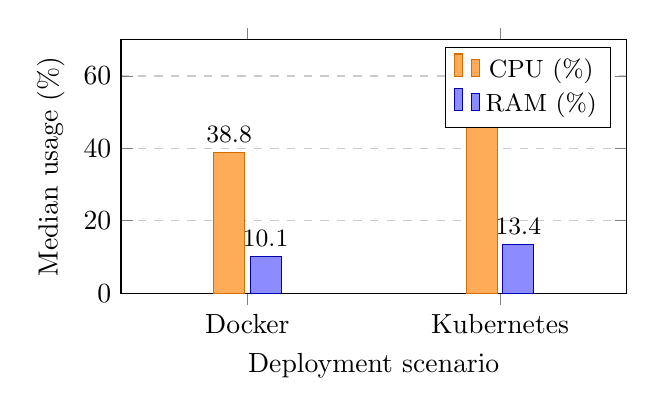
\begin{tikzpicture}
\begin{axis}[
  ybar, bar width=11.2pt,
  width=8cm, height=4.8cm,
  xlabel={Deployment scenario},
  ylabel={Median usage (\%)},
  symbolic x coords={Docker,Kubernetes},
  xtick=data,
  ymin=0, ymax=70,
  ymajorgrids=true, grid style={dashed,gray!40},
  legend style={at={(0.97,0.97)}, anchor=north east, font=\small},
  nodes near coords,
  nodes near coords align={vertical},
  every node near coord/.append style={font=\small},
  enlarge x limits=0.5,
]
\addplot[fill=orange!65, draw=orange!85!black]
  coordinates {(Docker,38.8) (Kubernetes,51.2)};
\addplot[fill=blue!45, draw=blue!70!black]
  coordinates {(Docker,10.1) (Kubernetes,13.4)};
\legend{CPU (\%), RAM (\%)}
    \end{axis}
\end{tikzpicture}
\end{center}
\caption{Median CPU and RAM consumption of \texttt{voctocore} in the two
instrumented scenarios with four active sources.\label{fig:cpu_ram}}
\end{figure}

Under peak load, the Docker Compose stack demonstrated high compute efficiency, consuming $38.8\%$ CPU and $10.1\%$ RAM. In comparison, the Kubernetes deployment exhibited an increased footprint, demanding $51.2\%$ CPU and $13.4\%$ RAM. This performance delta is primarily attributed to the co-located Minikube control plane sharing the host's hardware. The virtualization layer's management processes, state store, and local node monitoring introduce a fixed, non-negligible base load that remains independent of active media channels. In an enterprise-managed cloud deployment where the control plane is isolated on dedicated hardware infrastructure, this processing overhead would be circumvented.

Crucially, under Docker optimization, the CPU scaled linearly from $33.5\%$ with a single active camera to $38.8\%$ with four streams. This yields a marginal cost of just $1.8$ percentage points per additional high-definition source. This flat scaling curve validates the low-overhead data path provided by the GStreamer pipeline and confirms that local container network sharing effectively mitigates inter-container network stack bottlenecks.

\begin{table}[H]
\caption{System Performance and Resource Footprint Summary.}
\label{tab:perf}
\small
\begin{tabularx}{\textwidth}{XCCCC}
\toprule
\textbf{Deployment Scenario} & \textbf{CPU (\%)} & \textbf{RAM (\%)} & \textbf{Package Power (W)} & \textbf{Active Sources}\\
\midrule
Local & & & & \\
Docker         & 38.8 & 10.1 & 25--32 & 4 \\
Kubernetes  & 51.2 & 13.4 & 25--27\textsuperscript{a} & 4 \\
\bottomrule
\end{tabularx}
\noindent{\footnotesize{\textsuperscript{a} A single 36.1~W anomaly in the 3-source run was treated as an isolated baseline artefact due to transient host-level RAPL fluctuations.}}
\end{table}

Environmental and infrastructure efficiency was monitored using the Intel Running Average Power Limit (RAPL) hardware interfaces. As detailed in Table~\ref{tab:perf}, the peak processor package power draw reached $32\text{ W}$ in the Docker environment under full operational load. This power footprint represents less than $20\%$ of the processor's total Thermal Design Power ($\text{TDP} = 165\text{ W}$). This leaves extensive compute and thermal headroom on the 10-core host machine to accommodate downstream tasks such as real-time H.264/H.265 distribution encoding or multi-platform transcoding.

Interestingly, while Kubernetes registered a higher CPU utilization metric, its measured package power consumption remained remarkably close to the Docker baseline ($25\text{ W}$--$27\text{ W}$). This decoupling of CPU utilization from power draw indicates that the Kubernetes overhead is dominated by control-plane scheduling loops and context switches; because these processes do not trigger complex vector processing or intensive memory sub-system operations, they do not induce a proportional thermal or energy penalty in the physical package.

\subsection{Switching and Transition Latency Analysis}

To evaluate real-time responsiveness, source-switching latencies were benchmarked by cross-referencing command dispatch logs with immediate \texttt{CHANGE} telemetry confirmations. A rigorous sample size of $n=30$ discrete events was recorded for each containerized environment. Figure~\ref{fig:latency} shows the distribution of the measured latencies.

\begin{figure}[H]
\begin{center}
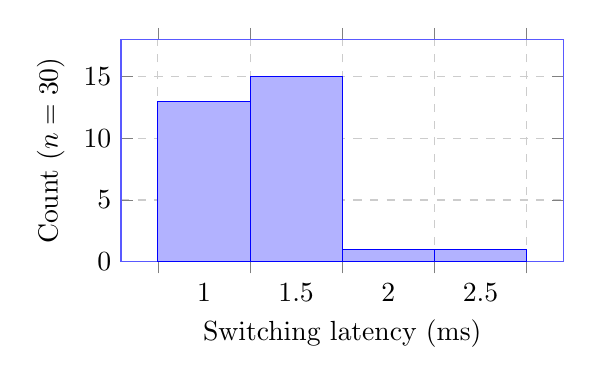
\begin{tikzpicture}
\begin{axis}[
  ybar interval, bar width=0.95,
  width=7.2cm, height=4.4cm,
  xlabel={Switching latency (ms)},
  ylabel={Count ($n=30$)},
  xtick={1.0,1.5,2.0,2.5,3.0},
  xmin=0.8, xmax=3.2,
  ymin=0, ymax=18,
  ymajorgrids=true, grid style={dashed,gray!40},
  fill=blue!35, draw=blue!65,
]
\addplot coordinates {(1.0,13) (1.5,15) (2.0,1) (2.5,1) (3.0,0)};
\end{axis}
\end{tikzpicture}
\end{center}
\caption{Distribution of source-switching latencies in the Docker Compose
scenario.\label{fig:latency}}
\end{figure}

The empirical distributions summarized in Table~\ref{tab:latency_summary} reveal that source-switching remains under $5\text{ ms}$ across both architectures, yielding a median latency of $1.50\text{ ms}$ in Docker Compose and $1.79\text{ ms}$ in Kubernetes. These values sit more than one order of magnitude below the strict $45\text{ ms}$ threshold established by the \textbf{ITU-R BT.1359-1 standard} for audio-to-video lip-sync desynchronization. Consequently, camera cuts are perceptually instantaneous to the audience.

\begin{table}[H]
\caption{Statistical Summary of Latency Performance (Source Cuts vs. Layout Transitions).}
\label{tab:latency_summary}
\small
\begin{tabularx}{\textwidth}{XCCCCC}
\toprule
\textbf{Metric Type} & \textbf{Deployment Topology} & \textbf{n} & \textbf{Median (ms)} & \textbf{p95 (ms)} & \textbf{Max (ms)}\\
\midrule
Source Switch        & Docker Compose & 30 & 1.50 & 2.30  & 2.70 \\
Source Switch        & Kubernetes     & 30 & 1.79 & 2.58  & 4.72 \\
Composite Transition & Docker Compose & 32 & 2.80 & 4.20  & 5.30 \\
Composite Transition & Kubernetes     & 32 & 78.93 & 87.14 & 104.16 \\
\bottomrule
\end{tabularx}
\end{table}

However, evaluating layout-driven composite transitions (e.g., animating an active scene into a Picture-in-Picture layout) revealed a structural divergence. While Docker handled these transitions smoothly with a median of $2.80\text{ ms}$, Kubernetes exhibited an elevated median of $78.93\text{ ms}$. This layout change operates on a $40\text{ ms}$ internal cycle tied to the frame rate. In the un-contended Docker environment, the pipeline processes the transition without missing a cycle. Conversely, the localized Minikube control plane induces sufficient scheduling contention that the GStreamer pipeline occasionally misses the immediate frame boundary, pushing the transition onset to the subsequent frame cycle. Because this metric dictates layout rendering fluidity rather than underlying stream alignment, lip-sync integrity remains completely uncompromised.

\subsection{System Resilience, Self-Healing and Long-Term Operational Stability}

The architecture's fault tolerance was stress-tested by abruptly terminating the primary process inside the active \texttt{cam1} ingest container via a destructive \texttt{kill -9} signal over 10 distinct iterations.

The containerized environment successfully demonstrated autonomous self-healing capabilities. The Docker Compose framework fully re-established the live camera feed into the program buffer in a median of $520\text{ ms}$. The Kubernetes pod structure handled the failover in $570\text{ ms}$. The marginal $50\text{ ms}$ latency penalty in Kubernetes represents the polling and observation cycle of the local \texttt{kubelet} supervisor before initiating container restart sequences. Crucially, throughout this recovery window, the isolated design of our stream-blanker module ensured that the mixer continuously broadcasted using the remaining active sources. The audience experiences no dropped signal, frozen software states, or stream termination, achieving automatic recovery in under a second without human operator intervention.

To guarantee the engineering viability of mixing real-time multimedia using an interpreted control layer (Python) over low-level C-libraries (GStreamer), continuous stress tests were performed for 31 minutes per scenario, compiling hundreds of distinct telemetry data points. Following transient initialization peaks, CPU allocation permanently stabilized within the $49\%\text{--}58\%$ band for Docker and the $54\%\text{--}60\%$ band for Kubernetes. More importantly, RAM allocation profiles remained entirely flat throughout the broadcast sessions, registering zero memory leaks or progressive state degradation. This empirical stability confirms that the system can reliably sustain baseline media operations without requiring periodic reboots or suffering performance decay.


%%%%%%%%%%%%%%%%%%%%%%%%%%%%%%%%%%%%%%%%%%
\section{Conclusions}
\label{sec:conclusions}

\subsection{Summary of main findings}

This paper has demonstrated that an enhanced, cloud-native remote video production architecture built upon an open-source framework can successfully meet the rigid demands of professional live broadcasting. By taking the open-source Voctomix 2.0 system as an architectural baseline, we have engineered an extension layer that introduces automated audio-follows-video (AFV) transitions, dynamic multi-layer alpha-channel overlays, and a clean, buffer-level stream-blanking module. These contributions prove that sophisticated, production-grade broadcast features can be modularly integrated on top of low-level mixing cores without compromising pipeline stability.

Our empirical results firmly validate the technical viability of this software-defined approach across three deployment tiers, ranging from a bare-metal local workstation up to a fully orchestrated Kubernetes cluster. The containerized stack successfully sustained a four-source 1080p25 uncompressed aggregate stream at a highly efficient compute footprint ($38.8\%$ CPU under Docker Compose) and minimal processor power draw ($25\text{ W}$--$32\text{ W}$). With a measured median source-switching latency of just $1.5\text{ ms}$, the system operates well within the strict $45\text{ ms}$ synchronization boundary mandated by the ITU-R BT.1359-1 recommendation. Long-term stress runs confirmed complete memory stability, while forced failure experiments proved the system’s robust self-healing nature, achieving automated recovery from camera crashes in under $600\text{ ms}$ without human operator intervention.

\subsection{Future Work}

Building upon the enhanced open-source architecture established in this study, several promising tracks emerge for future research:

\begin{itemize}    
    \item Native SRT Transport Layer Integration: Developing modular GStreamer ingest and egress plugins supporting Secure Reliable Transport (SRT) will allow the core mixer to seamlessly bind to public content delivery networks (CDNs) and cloud endpoints, moving beyond uncompressed local TCP networking.    
    \item Web-Native Control Plane (Cloud GUI): Transitioning from a GTK 3 desktop application to a browser-based, light-weight control web app will remove display-server dependencies. Operators will be able to handle remote live mixes securely from any standard thin-client or connected device.    
    \item Prometheus and Grafana Dashboard Observability: Leveraging the non-intrusive RabbitMQ AMQP telemetry stream, a custom exporter can easily expose real-time metrics (CPU, memory, packet status, active source states) to a Prometheus time-series database, enabling professional enterprise monitoring dashboards via Grafana with zero core overhead.    
    \item Asynchronous AI-Driven Transcription Overlays: The event-driven architecture can be expanded by routing the isolated program audio to a sidecar automatic speech recognition engine. The transcribed text can then be pushed back as instantaneous overlay subtitle commands, achieving real-time accessibility closed-captioning without human operator intervention.
\end{itemize}

%%%%%%%%%%%%%%%%%%%%%%%%%%%%%%%%%%%%%%%%%%
\vspace{6pt}

\authorcontributions{%
Conceptualization, M.H.S. and \'A.L.;
Methodology, M.H.S. and \'A.L.;
Software, M.H.S.;
Validation, M.H.S. and \'A.L.;
Formal analysis, M.H.S.;
Investigation, M.H.S.;
Writing---original draft preparation, M.H.S.;
Writing---review and editing, \'A.L., A.R.P. and D.J.B.;
Supervision, \'A.L., A.R.P. and D.J.B.;
Project administration, \'A.L.;
All authors have read and agreed to the published version of the manuscript.}

\funding{This work was carried out in the context of the CyberNEMO project,
funded by the European Union's Horizon Europe research and innovation programme
under grant agreement No.~101168182. Views and opinions expressed are however
those of the authors only and do not necessarily reflect those of the European
Union. Neither the European Union nor the granting authority can be held
responsible for them.}

\institutionalreview{Not applicable.}

\informedconsent{Not applicable.}

\dataavailability{The source code and deployment scripts supporting the results
of this article are publicly available in the project repository at
\url{https://github.com/martin1210235/voctomix-2.0}. The raw experimental logs
used to compute the reported metrics are available from the corresponding author
upon reasonable request.}

\acknowledgments{This project has received funding from two projects in the EU Horizon Europe research and innovation Programme under Grant Agreement No. 101070118 (NEMO project) and Grant Agreement No. 101168182 (CyberNEMO project).}

\conflictsofinterest{The authors declare no conflicts of interest. The funders
had no role in the design of the study; in the collection, analyses, or
interpretation of data; in the writing of the manuscript; or in the decision to
publish the results.}

\abbreviations{Abbreviations}{
The following abbreviations are used in this manuscript:\\

\noindent
\begin{tabular}{@{}ll}
AFV    & Audio Follows Video\\
AMQP   & Advanced Message Queuing Protocol\\
API    & Application Programming Interface\\
DMA    & Direct Memory Access\\
GTK    & GIMP Toolkit\\
JSON   & JavaScript Object Notation\\
K8s    & Kubernetes\\
OBS    & Open Broadcaster Software\\
PIP    & Picture in Picture\\
RAPL   & Running Average Power Limit\\
REMI   & Remote Integration Model\\
SBS    & Side by Side\\
SDI    & Serial Digital Interface\\
SRT    & Secure Reliable Transport\\
TCP    & Transmission Control Protocol\\
UDP    & User Datagram Protocol\\
UPM    & Universidad Polit\'ecnica de Madrid\\
\end{tabular}
}

%%%%%%%%%%%%%%%%%%%%%%%%%%%%%%%%%%%%%%%%%%
\begin{adjustwidth}{-\extralength}{0cm}

\reftitle{References}
\bibliography{references}

\PublishersNote{}
\end{adjustwidth}
\end{document}
